% \documentclass{article}
\documentclass[runningheads]{llncs}
\usepackage[spanish,english,portuguese]{babel}

% Set page size and margins
% Replace `letterpaper' with `a4paper' for UK/EU standard size
\usepackage[a4paper,top=2cm,bottom=2cm,left=3cm,right=3cm,marginparwidth=1.75cm]{geometry}
\usepackage{amsmath}
\usepackage{graphicx}
\usepackage[colorlinks=true, allcolors=blue]{hyperref}
\usepackage[utf8]{inputenc}
\usepackage{csquotes}
\usepackage{natbib}
\usepackage{url}
\usepackage{hyperref}
% \usepackage{footmisc}

\usepackage{color}

\def \bchregi {\begin{color}{red}} 
\def \echregi {\end{color}}

\def \bchgon {\begin{color}{blue}} 
\def \echgon {\end{color}}

\def \bchedel {\begin{color}{cyan}} 
\def \echedel {\end{color}}

\def \bwarn {\begin{color}{yellow}} 
\def \ewarn {\end{color}}

\providecommand{\keywords}[1]
{
  \small	
  \textbf{\textit{Keywords---}} #1
}

\title{Open Educational Research Data: Are Repositories Delivering?}
% \author{Gonzalo Torterolo-Silva - ORCID https://orcid.org/0009-0003-5004-0342}
% \author{Regina Motz - ORCID https://orcid.org/0000-0002-1426-562X}
% \author{Edelweis Rohrer - ORCID https://orcid.org/0000-0002-8257-5291}
% \institute{UdelaR}

\begin{document}
\selectlanguage{spanish}
\maketitle

\selectlanguage{spanish}
\begin{abstract}
%Este trabajo presenta un análisis que pretende aportar mayor claridad sobre el grado de cumplimiento de los repositorios de datos   
En el contexto digital actual, que tiene al movimiento de la ciencia abierta como un nuevo paradigma de producción y circulación de conocimiento, este trabajo analiza en qué medida los repositorios de datos de investigación responden a las necesidades técnicas, legales y éticas de los investigadores en educación y ciencias sociales. El abordaje se realiza aplicando un enfoque que combina tres actividades: revisión bibliográfica, entrevista a experto y análisis de catálogos de repositorios. De la fusión de los resultados obtenidos, se concluye que las características de los repositorios que resultan más valoradas por los investigadores de estas disciplinas son la reputación de los repositorios, facilidad de uso, disponibilidad de información de contexto, sostenibilidad (conservación de los datos a largo plazo), apoyo técnico y cumplimiento de los principios FAIR (que promueven la producción de datos Encontrables, Accesibles, Interoperables, Reutilizables). Además, este artículo profundiza en el rol que cumplen los catálogos de repositorios para facilitar la selección de repositorios adecuados para depositar los datos, proporcionando a los investigadores información útil para evaluar la calidad de los repositorios, en cuanto a si responden a sus necesidades.

Este estudio proporciona información valiosa para promover la adopción de prácticas de datos abiertos en el campo de la investigación educativa.



%Este artículo analiza los criterios que influyen en la selección de repositorios de datos de investigación por parte de investigadores educativos. Se destaca la creciente importancia del acceso público a los datos en el contexto de la ciencia abierta y se examinan los principios FAIR (Encontrables, Accesibles, Interoperables, Reutilizables) como guía para la gestión de datos. El estudio se basa en una metodología mixta, que incluye una revisión bibliográfica, una consulta a expertos y un análisis de catálogos de repositorios.
%La revisión bibliográfica identificó factores clave como la reputación del repositorio, la facilidad de uso, la disponibilidad de metadatos y el cumplimiento de los principios FAIR. La consulta a expertos enfatizó la importancia de los identificadores persistentes, la sostenibilidad y la interoperabilidad de los repositorios. El análisis de catálogos reveló que FAIRSharing se destaca por su curaduría y calidad de datos, mientras que re3data es una fuente primaria de información.
%El artículo concluye que los investigadores educativos necesitan herramientas y criterios claros para seleccionar repositorios adecuados. Se subraya la necesidad de repositorios que faciliten la interoperabilidad y que cuenten con apoyo institucional y asistencia técnica. El estudio proporciona información valiosa para promover la adopción de prácticas de datos abiertos en el campo de la investigación educativa.
      
% Finalmente, se destaca el rol del investigador como agente activo que colabora en la  democratización del conocimiento científico, promoviendo una cultura de datos abiertos en el ámbito educativo.\\
\end{abstract}
% Regi: 5 keywords de ERIC en espa`nol
% Gonzalo: No hay version en español de las keywords (ver por ej https://vocabularyserver.com/eric/index.php?tema=255&/archives), por lo que traduje a mi criterio
\keywords{herramientas-de-investigación, archivos, catálogos-en-linea, metadatos, uso-de-datos}


\selectlanguage{english}
\begin{abstract}
In today’s digital context, where the open science movement is emerging as a new paradigm for the production and dissemination of knowledge, this paper analyzes the extent to which research data repositories meet the technical, legal, and ethical needs of researchers in education and the social sciences. The study applies a mixed-methods approach combining three activities: a literature review, an expert interview, and an analysis of repository catalogs.

Based on the synthesis of the results, it is concluded that the most valued characteristics of repositories among researchers in these disciplines include repository reputation, ease of use, availability of contextual information, sustainability (long-term data preservation), technical support, and compliance with the FAIR principles (which promote the creation of data that are Findable, Accessible, Interoperable, and Reusable).

Furthermore, this article explores the role of repository catalogs in helping researchers select appropriate repositories for data deposit, by providing useful information to assess their quality and relevance to researchers’ needs.

This study provides valuable insights to support the adoption of open data practices in the field of educational research.

%This article discusses the criteria that influence the selection of research data repositories by educational researchers. It highlights the growing importance of public access to data in the context of open science and examines the FAIR (Findable, Accessible, Interoperable, Reusable) principles as a guide for data management. The study is based on a mixed methodology, including a literature review, expert consultation and analysis of repository catalogs.
%The literature review identified key factors such as repository reputation, ease of use, metadata availability, and compliance with FAIR principles. Expert consultation emphasized the importance of persistent identifiers, sustainability and interoperability of repositories. Catalog analysis revealed that FAIRSharing stands out for its curation and data quality, while re3data is a primary source of information.
%The article concludes that educational researchers need clear tools and criteria for selecting appropriate repositories. It stresses the need for repositories that facilitate interoperability and that have institutional support and technical assistance. The study provides valuable information to promote the adoption of open data practices in the field of educational research.
\end{abstract}
% 5 keywords de ERIC
% https://vocabularyserver.com/eric/index.php?tema=6128&/research-tools
% https://vocabularyserver.com/eric/index.php?tema=255&/archives
% https://vocabularyserver.com/eric/index.php?tema=3223&/online-catalogs
% https://vocabularyserver.com/eric/index.php?tema=4001&/metadata
% https://vocabularyserver.com/eric/index.php?tema=5348&/data-use
\keywords{research-tools, archives, online-catalogs, metadata, data-use}


\selectlanguage{portuguese}
\begin{abstract}
No atual contexto digital, em que o movimento da ciência aberta se consolida como um novo paradigma de produção e circulação do conhecimento, este trabalho analisa em que medida os repositórios de dados de pesquisa atendem às necessidades técnicas, legais e éticas dos pesquisadores em educação e ciências sociais. A abordagem utilizada combina três atividades: revisão bibliográfica, entrevista com especialista e análise de catálogos de repositórios.

A partir da síntese dos resultados obtidos, conclui-se que as características mais valorizadas pelos pesquisadores dessas disciplinas são: a reputação dos repositórios, a facilidade de uso, a disponibilidade de informações contextuais, a sustentabilidade (preservação dos dados a longo prazo), o suporte técnico e o cumprimento dos princípios FAIR (que promovem a produção de dados Encontráveis, Acessíveis, Interoperáveis e Reutilizáveis).

Além disso, o artigo aprofunda o papel dos catálogos de repositórios na facilitação da escolha de repositórios adequados para o depósito de dados, oferecendo aos pesquisadores informações úteis para avaliar a qualidade dos repositórios em relação às suas necessidades.

Este estudo fornece informações valiosas para promover a adoção de práticas de dados abertos no campo da pesquisa educacional.

%Este artigo discute os critérios que influenciam a seleção de repositórios de dados de pesquisa por pesquisadores educacionais. Ele destaca a importância crescente do acesso público aos dados no contexto da ciência aberta e examina os princípios FAIR (Findable, Accessible, Interoperable, Reusable) como um guia para o gerenciamento de dados. O estudo baseia-se em uma metodologia mista, incluindo uma revisão da literatura, uma consulta a especialistas e uma análise de catálogos de repositórios.
%A revisão da literatura identificou fatores importantes, como a reputação do repositório, a facilidade de uso, a disponibilidade de metadados e a conformidade com os princípios FAIR. A consulta a especialistas enfatizou a importância dos identificadores persistentes, da sostenibilidade e da interoperabilidade dos repositórios. A análise dos catálogos revelou que o FAIRSharing se destaca por sua curadoria e qualidade de dados, enquanto o re3data é uma fonte primária de informações.
%O artigo conclui que os pesquisadores educacionais precisam de ferramentas e critérios claros para selecionar os repositórios adequados. Ele destaca a necessidade de repositórios que facilitem a interoperabilidade e que tenham apoio institucional e assistência técnica. O estudo fornece informações valiosas para promover a adoção de práticas de dados abertos no campo da pesquisa educacional.
\end{abstract}
\keywords{ferramentas-de-pesquisa, arquivos, catálogos-online, metadados, uso-de-dados}

\selectlanguage{spanish}
\section{Introducción}
\label{intro}
En la era digital actual, el movimiento de ciencia abierta ha reconfigurado profundamente los paradigmas de producción y circulación del conocimiento científico. Dentro de este marco transformador, el acceso público a los datos de investigación emerge como un componente estratégico fundamental, particularmente en el campo educativo. \  La aplicación de estos paradigmas no solo robustece los pilares de transparencia y reproducibilidad que sustentan el método científico \citep{OECD2020}, sino que además facilita el análisis secundario y contribuye al impacto social del conocimiento \citep{ec2016, wilkinson2016}. Los beneficios potenciales son particularmente significativos en el ámbito educativo, donde la posibilidad de contrastar resultados entre diferentes contextos socioculturales y sistemas pedagógicos podría generar insumos para la evolución de las políticas públicas en educación. 

La \citet[p.~10]{unesco2021} conceptualiza los datos abiertos de investigación como aquellos que deben estar ``disponibles de manera oportuna, en un formato fácil de utilizar, legible y modificable por personas y máquinas'', articulándose bajo los principios FAIR (Fáciles de encontrar, Accesibles, Interoperables y Reutilizables) \citep{wilkinson2016}.  La disponibilidad de repositorios alineados con estos principios facilita la tarea de los investigadores, tanto para depositar como para reusar datos. Sin embargo, no es trivial decidir en qué repositorio depositar, organizar y gestionar los datos de investigación. En este sentido, los principios TRUST \citep{Lin2020TRUST} representan un marco de referencia muy valioso para evaluar la calidad de los repositorios científicos,  promoviendo la Transparencia (políticas de uso claras), Responsabilidad (en lo que refiere a la gestión de las colecciones de datos), el foco en el Usuario (disponibilidad de  herramientas para explorar, ubicar y reusar datos), Sostenibilidad (disponibilidad de los servicios de acceso a los datos  a largo plazo) y Tecnología (uso e implementación de estándares y herramientas adecuadas para la gestión y curación de los datos).
La exhaustiva caracterización de \citet{behnke_2020_5361952} detalla cómo estos principios  incluyen tanto requerimientos organizacionales (como políticas claras de gestión de datos y soporte para formatos estándar) como técnicos (desde metadatos granularizados hasta sistemas de identificadores persistentes).  \\


La organización y agrupación de colecciones de datos de investigación en repositorios responde a diferentes criterios de acuerdo a los cuales es posible categorizar los repositorios como disciplinares, cuando contienen datos 
de un área específica de conocimiento, generalistas, en caso contrario, y también institucionales, en caso de albergar datos de una institución en particular. %o no,  y entre repositorios institucionales o huérfanos (contienen datos que no pertenecen a una institución en particular). 
A su vez, en algunas disciplinas, por ejemplo economía o epidemiología, la mayor parte de los datos gestionados son cuantitativos, mientras que en otras, como las ciencias sociales y la educación, los datos son en su mayor parte cualitativos. Cada una de estas categorías de repositorios puede requerir la priorización de algunos principios sobre otros, o el uso de diferentes estándares o tecnologías para su implementación. En general, los datos de investigación de una misma disciplina tienen características en común, por lo que los requerimientos tecnológicos son similares. %Por ejemplo, en algunas disciplinas los datos deben estar actualizados en todo momento, por lo que van a usar los mismos a estándares de metadatos. 
%ACA DECIR que en general los datos de una misma disciplina son de naturaleza similar (es verdad?), por ejemplo requieren del mismo tipo de metadatos (por ejemplo datos que deben estar siempre actualizados....o lo que más importa es la reputación de la fuente), entonces la plataforma tecnológica va a tener los mismos requerimientos....
En particular, la investigación educativa enfrenta obstáculos específicos, especialmente cuando se trabaja con datos cualitativos que, como destaca \citet{antonio}, demandan niveles excepcionales de contextualización y mecanismos especializados de protección ética, implementados con tecnologías específicas, que muchos repositorios generalistas no están preparados para ofrecer.   
Otros estudios como el de \citet{strecker_disappearing_repos_23} informan sobre los riesgos de estos repositorios para cumplir con los estándares de calidad, indicando además que los repositorios disciplinares afines a humanidades y ciencias sociales son de los más afectados por este tipo de problemas. Otros autores, como \citet{google_dataset_aglomeration, Gerasimov2024} también advierten sobre tendencias de centralización de la mayoría de los datasets sobre el conjunto de repositorios generalistas. Paradójicamente, varias recomendaciones de estos repositorios generalistas alientan a los investigadores a utilizar repositorios disciplinares e institucionales \citep{barbosa_2024_11105430}.
En particular, los trabajos de \citet{Jia25} y \citet{avila2024} destacan por su análisis exhaustivo de las pautas para seleccionar repositorios de datos científicos confiables. 
También organismos internacionales como la \citet{unesco2021} y la \citet{OECD2020}, alineados con los principios FAIR y TRUST, han impulsado políticas que fomentan el uso de repositorios digitales especializados para el almacenamiento, preservación y diseminación ética de datos científicos.

Como argumentan \citet{borgman2018}, estas infraestructuras digitales han dejado de ser meros almacenes de información para convertirse en nodos fundamentales de las redes contemporáneas de producción de conocimiento, facilitando no solo el acceso sino también la interoperabilidad y el enriquecimiento progresivo de los datasets mediante sucesivas reutilizaciones. En esta misma línea, la reciente conceptualización de \citep[p.~27]{avila2024} enfatiza su rol como sistemas dinámicos que permiten ``almacenar, organizar, recuperar y acceder a conjuntos de datos de diversa naturaleza temática y tipológica'', constituyéndose así en motores esenciales para la ciencia abierta. \\

La aplicación de los principios FAIR \citep{wilkinson2016} y TRUST \citep{Lin2020TRUST} enfrentan retos particulares en disciplinas como la educación y las ciencias sociales, donde la heterogeneidad, sensibilidad y complejidad de los datos dificultan la estandarización y la creación de infraestructuras especializadas, alineadas con los requerimientos de estas disciplinas. Sin embargo, la escasez de repositorios disciplinares en estas áreas, sumada a desafíos éticos, legales y culturales, obliga a los investigadores a recurrir mayoritariamente a repositorios institucionales o generalistas, que no siempre satisfacen los requerimientos específicos para la gestión óptima de datos educativos y sociales.

Como advierte \citet{borgman2016} en su análisis sobre las ecologías del conocimiento, los datos solo alcanzan su pleno valor científico cuando se integran en ecosistemas robustos que articulen coherentemente dimensiones técnicas, prácticas comunitarias e institucionales. Precisamente, esta articulación presenta desafíos particulares en el ámbito educativo y de ciencias sociales, donde la disponibilidad de repositorios disciplinares especializados es escasa en comparación con otras áreas del conocimiento \citep{kraehmer2023,Lamb2024}. Esta disparidad resulta paradójica si consideramos la complejidad intrínseca de los datos educativos, que abarcan desde mediciones cuantitativas estandarizadas hasta registros etnográficos profundamente contextualizados, frecuentemente conteniendo información sensible (por ej. sobre menores de edad en entornos escolares específicos \citep{gomes2022}).\\

Frente a estos desafíos, iniciativas como re3data \citep{pampel2013} han buscado crear catálogos integrados que faciliten la localización y evaluación de repositorios especializados. La selección informada de repositorios se vuelve entonces un desafío crucial. Los catálogos de repositorios emergen como herramientas clave para buscar, filtrar y evaluar opciones según criterios técnicos, éticos y disciplinares. 

Sin embargo, en lo que refiere a repositorios de datos de investigaciones en educación, se observa una muy escasa presencia disciplinar. A modo de ejemplo, de acuerdo a la información recabada en junio de 2025, los catálogos FAIRSharing, DataCite Commons y re3Data tienen registrados en total 1252, 1767 y 3259 repositorios respectivamente, de los cuales únicamente 22, 5 y 47 corresponden a repositorios de datos de investigación en el área de la educación.

En este sentido, creemos que este trabajo aporta en prestar atención a las necesidades de los investigadores de la educación, para continuar mejorando el servicio que los repositorios pueden ofrecerles, para incentivar así su desarrollo.

Este artículo analiza las necesidades para la publicación de datos en educación y ciencias sociales, y las características  de los repositorios más valorados por las investigadoras y los investigadores de estas disciplinas, considerando sus preocupaciones éticas, técnicas y legales. Además, este trabajo explora el papel de los catálogos de repositorios en la selección de repositorios como toma de decisiones informadas, con el objetivo de fortalecer la cultura de datos abiertos y contribuir al avance de la ciencia abierta en estas disciplinas.\\

\section{Metodología}
\label{Metodo}
Para la realización de este estudio se siguió un diseño metodológico de enfoque secuencial exploratorio con las siguientes tres fases interrelacionadas: Revisión Bibliográfica, Entrevista a Experto y Análisis de Catálogos.

\paragraph{Objetivo:} Identificar cómo responden los repositorios a las preocupaciones  éticas, técnicas y legales que tienen las investigadoras y los investigadores en el momento de depositar datos de investigaciones educativas.

\paragraph{Fases Metodológicas}
\begin{itemize}
    \item [a)] Revisión Bibliográfica
    
Fuentes: Artículos en Scopus/WoS/ (keywords: "open data" + "education research" + "concerns"), informes de UNESCO y OECD. Criterios de exclusión: trabajos sobre repositories de recursos educativos abiertos y trabajos que solo consideran el acceso abierto a publicaciones de investigación.

Análisis: Codificación asistida con Elicit \footnote{Asistente de investigación con IA: https://elicit.com/} para categorizar preocupaciones recurrentes (ej. privacidad, propiedad intelectual, esfuerzo adicional).

Resultado esperado: Mapa conceptual de barreras documentadas en la literatura (2015–2025).

\item [b)]  Entrevista a Experto

Participante: Responsable del repositorio de datos abiertos de la Agencia Nacional de Investigación e Innovación (ANII) de Uruguay.

Protocolo: Entrevista semiestructurada (30–45 min) 

Análisis: Transcripción y codificación para rectificar o ratificar categorías revisadas en la literatura.

\item [c)] Análisis de Catálogos de Repositorios

    Muestra:  6 Catálogos de amplio uso internacional(OpenDOAR, ROAR, OpenAIR, Figshare,DataCite Commons
    
    Variables evaluadas: actividad del repositorio, creación de identificadores persistentes, soporte para especificar el contexto, cumplimiento de estándares para interoperabilidad,  adhesión a políticas de licenciamiento y sostenibilidad.

\end{itemize}

\paragraph{Triangulación y Validación:}
 La combinación de estos tres métodos, revisión bibliográfica, consulta a experto y análisis de catálogos, permitió triangular la información, aumentando la validez y confiabilidad de los resultados.

\section{Resultados}

Esta sección presenta los resultados obtenidos a partir de la revisión bibliográfica, la consulta a expertos y el análisis de catálogos de repositorios.

\subsection{Resultados de revisión bibliográfica}

Numerosos estudios se han centrado en identificar los factores que impactan en la voluntad de los investigadores en compartir sus datos en abierto y se ha hecho un esfuerzo por destacar algunos de ellos aquí, especialmente desde la perspectiva de los repositorios. 
La revisión bibliográfica realizada muestra que los estudios abarcan encuestas, revisiones sistemáticas de la literatura, meta-análisis, grupos focales y mesas redondas, de las más actuales \citep{tenopir2011,revision2020,barczak2022,casali2022open, researchers2022,borycz2023,logan2021,researchers2024,malasya,bio-uy}. Es interesante observar que los estudios son con investigadores de distintas disciplinas, distinto nivel de expertise y de diferentes contextos geográficos. Curiosamente, pocos de estos estudios se han realizado con investigadores de Ciencias de la Educación. Entre los más destacados que involucran opiniones de investigadores relacionados con la disciplina Educación encontramos el trabajo de \citet{casali2022open} que analiza una encuesta administrada a investigadores de la comunidad LACLO (Conferencia Latinoamericana de Tecnologías de Aprendizaje) y los trabajos de \citet{logan2021} y de \citet{guia} 
que presentan guías sobre publicación de datos abiertos expresamente dirigidas para investigadores en Educación.\\

Mientras que el trabajo de \citet{casali2022open} destaca barreras como el tiempo y el esfuerzo requeridos para compartir los datos, la falta de financiamiento para la estandarización de los datos y las restricciones relacionadas con la seguridad y la confidencialidad de los datos, observamos que en los trabajos de \citet{logan2021, guia} se presta especial atención a los procedimientos para mantener la seguridad y la confidencialidad de los datos, evidenciando que este constituye un problema en común.\\

La mayoría de los trabajos coinciden en reconocer como aspectos importantes en la problemática planteada por los investigadores el esfuerzo extra que significa curar los datos para su publicación en abierto.  Mientras en general se atribuye esta problemática al desarrollo de los repositorios poco centrados en el usuario, para otros autores como \citet{borycz2023} y \citet{casali2022open}, se debe a la falta de apoyo administrativo a los investigadores en la preparación de los datos.\\

Otros estudios, como el de \citet{grattarola2024gaps} y \citet{ mabile2025recommendations}, señalan que la desmotivación principal para compartir los datos en abierto  recae en la falta de incentivos institucionales y la falta de reconocimiento por la publicación de datos.
Respecto al caso específico de datos procedentes de investigaciones cualitativas, se destaca en todos los trabajos la problemática de contar con elementos que permitan especificar el contexto en el cual los datos fueron obtenidos y la preocupación por contar con curaduría específica para asegurar el resguardo del investigador ante el problema legal y ético de uso de datos sensibles.\\

Los investigadores cualitativos en el área de ciencias sociales mencionan temas relativos a la privacidad de sus datos y el compromiso ético que implica su publicación. En ciencias sociales, los datos suelen involucrar personas, y aunque se anonimicen, muchos investigadores temen que los participantes puedan ser reidentificados, especialmente en comunidades pequeñas o temas sensibles \citep{kraehmer2023}. A pesar de existir mecanismos para mitigarlo, como el consentimiento informado, la responsabilidad de los repositorios en cuanto a la custodia de los datos no siempre resulta fácil de comprender para los productores de datos \citep{prosser2022}.\\

Estudios recientes como el de \citet{Lamb2024} ratifican algunos desafíos propios de las investigaciones cualitativas. Los investigadores cualitativos destacan que los datos (como entrevistas o diarios de campo) necesitan un conocimiento contextual profundo para ser interpretados adecuadamente cuando otros investigadores deciden reusar el dataset. \\

\subsection{Resultado consulta a experto}

Las conclusiones derivadas de la entrevista con el experto se basan en un estudio interno realizado por la Agencia Nacional de Investigación e Innovación (ANII). Este estudio, aunque no publicado, proporcionó información valiosa sobre las perspectivas de los investigadores en el contexto de Uruguay.
El estudio de la ANII reveló que los investigadores tienden a percibirse principalmente como consumidores de datos, más que como productores. Esta percepción influye en sus expectativas y necesidades en relación con los repositorios de datos.
El experto entrevistado, basándose en los resultados del estudio, destacó tres características clave que los investigadores consideran esenciales al momento de publicar sus datos:
\begin{itemize}
    \item \textbf{Asignación de identificadores persistentes}: La asignación de identificadores únicos y permanentes, preferentemente DOI, es vista como un requisito fundamental, especialmente debido a que muchas revistas científicas los exigen para la evaluación y citación de artículos.
    \item \textbf{Sostenibilidad y perdurabilidad}: La capacidad del repositorio para garantizar la conservación de los datos a largo plazo es considerada crucial para asegurar su disponibilidad y reutilización futura.
    \item \textbf{Interoperabilidad}: La capacidad del repositorio para facilitar la integración y el intercambio de datos entre diferentes plataformas y sistemas es valorada como esencial para maximizar el impacto y la reutilización de los datos.
\end{itemize}

La modalidad semiestructurada de la entrevista facilitó la exploración profunda de temas relevantes, sin restringir la espontaneidad del diálogo, lo que contribuyó a validar y ampliar los resultados del relevamiento bibliográfico con evidencia empírica y experiencia directa.

\subsection{Resultado del análisis de catálogos de repositorios}
Los estudios de \citep{witt_2024_11221855} y \citep{Jia25} establecen los principales criterios para evaluar repositorios de datos de investigación; no obstante, señalan que los investigadores enfrentan obstáculos para verificar el cumplimiento de dichos criterios, dada la escasa accesibilidad de esta información a priori. Esta limitación dificulta la selección de un repositorio adecuado para la publicación y la reutilización de datos. En este trabajo, analizamos el papel de los catálogos de repositorios en la difusión eficiente de dicha información, tomando como referencia los criterios definidos por estos autores y los desarrollados en el Data Repository Attributes Working Group\footnote{\url{https://www.rd-alliance.org/groups/data-repository-attributes-wg/}}.
Las características que buscamos identificar son; actividad del repositorio, creación de identificadores persistentes, soporte para especificar el contexto, cumplimiento de estándares para interoperabilidad y adhesión a políticas de licenciamiento y sostenibilidad.

\subsection*{Actividad del repositorio}
Los factores de actividad del repositorio y especificidad disciplinar  determinan fuertemente el impacto en la visibilidad y la reutilización de los datos. 
La actividad reciente del repositorio es un indicador clave de su confiabilidad. Son indicadores de actividad la frecuencia de actualizaciones (ej., nuevos datasets depositados mensualmente), fecha del último dataset depositado (evitar repositorios sin actividad en los últimos 12 meses), estadísticas públicas (ej., número de descargas o citas en DataCite).\\
%La Fig.~\ref{fig:datacite_commons_histograma} muestra el histograma de uso de un repositorio en DataCite.

Por otro lado, un repositorio especializado en un área temática ofrece la ventaja significative de utilizar esquemas de metadatos específicos (ej. DDI \footnote{\url{https://ddialliance.org/}} para ciencias sociales), lo que mejora la interoperabilidad y el descubrimiento de los datos. Además, los repositorios temáticos atraen a usuarios especializados, lo que incrementa el impacto y la citación del dataset.


\subsection*{Creación de identificadores persistentes} 

El Identificador Digital de Objeto (DOI, por sus siglas en inglés) desempeña un papel fundamental en los repositorios de datos de investigación, ya que garantiza la localización, citación y preservación permanente de los conjuntos de datos. Proporciona un enlace único y estable, evitando la pérdida de datos debido a cambios en las URL o la desactualización de repositorios. Esto asegura que los conjuntos de datos permanezcan accesibles a largo plazo, cumpliendo con los principios FAIR. Al integrarse con sistemas de gestión bibliográfica (como Crossref o DataCite), el DOI permite vincular conjuntos de datos con artículos científicos, mejorando su visibilidad y facilitando el seguimiento de su impacto.

El DOI (Digital Object Identifier) es asignado por agencias registradoras autorizadas, siendo DataCite la más utilizada para datos de investigación o por repositorios/instituciones afiliadas a DataCite. En algunos casos puede ocurrir que un mismo dataset termine teniendo múltiples DOIs. Esto puede ocurrir si un investigador carga el mismo dataset en distintos repositorios y cada uno le asigna un DOI distinto, o en caso de actualizaciones o versiones, ya que algunos repositorios generan un nuevo DOI para versiones corregidas o ampliadas del mismo dataset. Esto no es deseable ya que las citas al dataset se dispersan entre varios DOIs, subestimando su impacto real y además se dificulta identificar cuál es la versión más actualizada. Para evitar estos problemas se recomienda priorizar el uso de repositorios de referencia en cada disciplina (ej. ICPSR en ciencias sociales) para evitar duplicaciones. En caso de esto no ser posible, las soluciones recomendadas son usar repositorios que admitan versiones bajo un mismo DOI y vincular DOIs alternativos mediante metadatos (relaciones \emph{isVersionOf} o \emph{isIdenticalTo} en esquemas como Schema.org). 

\subsection*{Soporte para documentar el contexto}

El contexto de un dataset incluye detalles sobre su origen, metodología con la cual fue generado, uso potencial y limitaciones. Los repositorios recolectan la información de contexto a través de metadatos descriptivos, documentación técnica (como Protocolos de laboratorio, cuestionarios o scripts de procesamiento), documentos adicionales (como Readme, Guías e Informes) y publicaciones vinculadas (DOI de artículos relacionados que usaron/citaron el dataset). \\


En los metadatos descriptivos al menos se debe informar:  
\begin{itemize}
\item Origen: Quién lo creó (Institución, proyecto de investigación, autoría) y Cobertura temporal/geográfica (Cuándo y dónde se generó el dataset) 
\item Propósito: Objetivo de la recolección 
\item Métodos de recolección: Instrumentos, protocolos o software utilizados 
\item Licencias y restricciones: Condiciones de uso (CC-BY, GDPR, acceso restringido).
\end{itemize}

Los catálogos como OpenAIRE y DataCite Commons fomentan el uso de estándares internacionales (como el protocolo OAI-PMH y metadatos FAIR), lo que asegura que los datos sean fácilmente localizables, accesibles y reutilizables por diferentes plataformas y sistemas, favoreciendo la colaboración y el intercambio de información entre comunidades científicas. Esta buena práctica de usar vocabularios controlados
y ontologías disciplinares (por ej.:  OECD Education Taxonomy) para facilitar la interoperabilidad es impulsada por FAIRsharing  ofreciendo entre sus funcionalidades un directorio curado de estándares de metadatos. Cuando un repositorio se indexa  en FAIRsharing, éste evalúa y recomienda estándares de metadatos específicos según su disciplina. \\

\subsection*{Adhesión a políticas}
Otro de los aspectos a considerar de un repositorio, que dependen de factores políticos o legales, son sus políticas de uso y de preservación o sostenibilidad. 
El problema de repositorios que se extinguen es un problema grave como reportan \citet{strecker_disappearing_repos_23}.
Algunos catálogos, como FAIRSharing, facilitan la evaluación de estos factores, permitiendo identificar la relación entre las políticas específicas de cada repositorio con políticas más generales.\\
Si tomamos el ejemplo de la NIH\footnote{\url{https://www.nih.gov/}} como financiador, este podría imponer el cumplimiento de sus términos de uso de datos \footnote{\label{nih_policy_fairsharing} 2023 Final NIH Policy for Data Management and Sharing - \url{https://fairsharing.org/FAIRsharing.7861ef}}. FAIRSharing es capaz de desplegar los repositorios compatibles con esta política, visualizados mediante el grafo de la Fig.~\ref{fig:fairsharing_nih_policy_repo_usages}. De esta forma, un investigador con un proyecto financiado por NIH puede limitar la selección del repositorio a utilizar por los encontrados en la consulta que produce el grafo de la Fig. ~\ref{fig:fairsharing_nih_policy_repo_usages}.\\


\begin{figure}[h]
    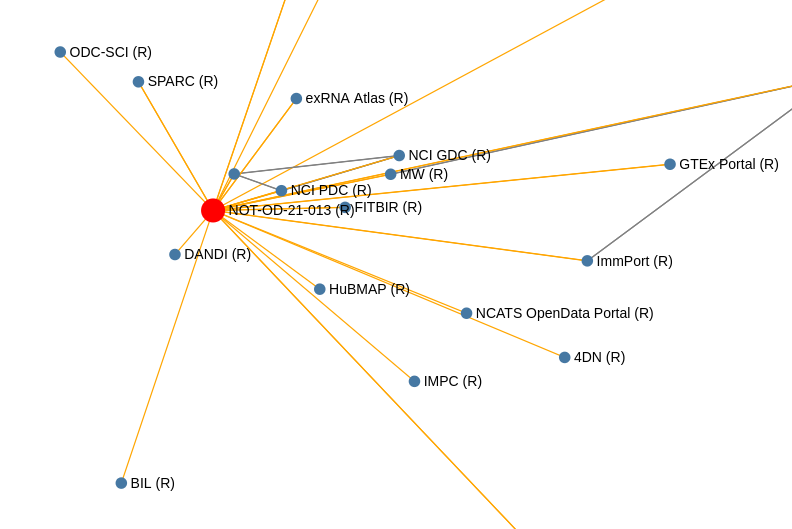
\includegraphics[width=0.5\textwidth]{img/FAIRSharing_NIHPol_Repos.png}
    \caption{
    Grafo de repositorios que utilizan la política del NIH - FAIRSharing - Obtenido el 26/06/2025
    }
    \label{fig:fairsharing_nih_policy_repo_usages}
\end{figure}

Otro mecanismo que aporta en la identificación de las adhesiones de los repositorios a ciertas políticas de uso y de sostenibilidad son las \emph{Certificaciones}. Las certificaciones de repositorios son mecanismos de evaluación externa que garantizan que un repositorio cumple con estándares de calidad, preservación y buenas prácticas en la gestión de datos. Las certificaciones son especialmente útiles para visualizar si los repositorios cumplen con políticas de preservación o sostenibilidad. Por ejemplo, un repositorio con alguna certificación indica que debió demostrar alguna de estas funcionalidades: asigna DOIs, usa esquemas de metadatos disciplinares,  cuenta con una infraestructura técnica sostenible (backups, migración de formatos), ofrece gestión de versiones para el control de cambios en los datasets, tiene un soporte técnico para dar respuesta a incidencias y que está respaldado por una institución estable (universidad, organismo público). Distintos sellos de certificaciones evalúan diferentes funcionalidades. Por ejemplo, un repositorio con certificación CoreTrustSeal \footnote{\url{https://www.coretrustseal.org}} está verificado para los criterios de asignación de DOI y preservación por un período mayor a 10 años, mientras que con un sello ISO 16363 \footnote{\url{https://www.iso.org/standard/87472.html}} tiene una verificación exhaustiva en los criterios de cumplimiento legal (ej., GDPR, propiedad intelectual) pero no en asignación de DOI.\\


Los catálogos recopilan datos de organismos certificadores y estandarizan la visualización de certificaciones para facilitar la comparación. Por ejemplo, re3data muestra el año de certificación y su vigencia.  FAIRsharing no certifica, pero evalúa y recomienda repositorios que adhieren al uso de estándares de metadatos y a principios FAIR. Además incluye un filtro por certificación (ej., CoreTrustSeal, ISO 16363) y proporciona enlaces a los informes de certificación oficiales. Un investigador que busca un repositorio para datos de educación puede usar FAIRsharing y filtrar por CoreTrustSeal y verificar en re3data si el repositorio tiene certificación vigente.

\subsection*{Compatibilidad de los repositorios con servicios}
Conocer la capacidad del repositorio para proveer o integrarse con ciertos servicios especializados en el área de investigación, así como las condiciones bajo las cuales los provee (precio del servicio o el nivel de disponibilidad del servicio), puede resultar relevante para los investigadores.  
Para enumerar algunos de estos servicios y funcionalidades se pueden mencionar la capacidad de realizar o recibir revisiones formales, la posibilidad de establecer períodos de embargo, asistencia técnica especializada o la disponibilidad de servicios de curaduría disciplinar.\\
En particular, para el caso de repositorios de datos de investigación cualitativos, la presencia o integración de servicios como anonimización, o mecanismos de control de acceso resulta valiosa para los investigadores. 
Catálogos como OpenAIRE ofrecen información sobre la integración de los diferentes repositorios con el ecosistema de servicios de la EOSC por ejemplo con el filtro ``Compatibility Level''  se pueden visualizar el nivel de compatibilidad del repositorio con servicios como : Amnesia\footnote{\url{https://www.openaire.eu/amnesia-guide}} servicio de anonimización, OpenAIRE AAI \footnote{\url{https://catalogue.openaire.eu/service/openaire.aai/overview}} API para servicio de acceso, Argos \footnote{\url{https://catalogue.openaire.eu/service/openaire.argos/overview}} servicio de Plan de Gestión de Datos, entre otros.  \\


El Cuadro~\ref{tab:catalog_main_features} ofrece un resumen de las principales características de los catálogos de repositorios revisados.



%*********************************************
%Muchos de estos catálogos promueven el uso de estándares comunes en la descripción de repositorios y datos, lo cual facilita el descubrimiento automatizado de los repositorios y sus datasets, su vinculación con publicaciones científicas y la construcción de infraestructuras digitales integradas. \\
%********************************************

%Los catálogos como OpenAIRE y DataCite Commons fomentan el uso de estándares internacionales (como el protocolo OAI-PMH y metadatos FAIR), lo que asegura que los datos sean fácilmente localizables, accesibles y reutilizables por diferentes plataformas y sistemas, favoreciendo la colaboración y el intercambio de información entre comunidades científicas.\\

%Un aporte importante de los catalogos es que certifican repositorios: Evalúan criterios como interoperabilidad, licencias claras y metadatos estructurados (ej: FAIRsharing asigna sellos de cumplimiento FAIR).\\


%Se llevó a cabo un análisis comparativo de los principales catálogos de repositorios de datos, con el objetivo de evaluar las características técnicas, organizativas y funcionales que los catálogos permiten conocer sobre los repositorios. 

%Algunas de estas características (certificaciones, sostenibilidad) se comprenden mucho mejor mediante estos catálogos de repositorios. 
%Otras características, como resumen de los contenidos de cada repositorio, pueden conocerse en cada caso, pero son presentadas de manera centralizada por los catálogos para una comparativa efectiva.\\


%Se analizaron los siguientes catálogos:
%\begin{itemize}
%    \item 
%    \emph{OpenDOAR}: Directorio global de repositorios de acceso abierto que ofrece acceso a recursos y productos académicos, incluyendo repositorios de datos.
%    \item
%    \emph{ROAR}: Registro de repositorios de acceso abierto, incluyendo repositorios de investigación además de otro tipo de repositorios como gubernamentales.
%    \item
%    \emph{OpenAIRE}: Servicio que interconecta varios catálogos y proporciona información sobre las relaciones entre repositorios, autores, instituciones y agencias de financiación. Se especializa informar sobre las integraciones de los repositorios con los servicios pertenecientes a la EOSC\footnote{European Open Science Cloud - \url{https://open-science-cloud.ec.europa.eu/}}, el entorno de investigación europeo abierto por excelencia.
%    \item 
%    \emph{FAIRsharing}:  Portal web que describe repositorios, estándares y políticas de datos, con un enfoque en los principios FAIR.
%    \item 
%    \emph{DataCite Commons}: Portal web que integra información sobre repositorios de investigación de diversa índole, y destaca por proveer información relativa al contenido de los mismos de manera sintética.
%    \item 
 %   \emph{Re3data}: Registro global de repositorios de datos de investigación de diferentes disciplinas académicas.
%\end{itemize}

\small
\begin{table}[h]
\centering
    \begin{tabular}{l | p{11cm}}
    \emph{Catálogo} & \emph{Características}\\
    \hline
    OpenDOAR & Permite conocer información básica del repositorio. \\ \hline
    ROAR &  Similar a  OpenDOAR, pero permite conocer la disciplina asociada al repositorio. Especializado en repositorios de publicaciones académicas, contiene repositorios de datos de investigacion de manera casual. \\ \hline
    Re3data & Se especializa en describir repositorios de datos de investigación. Provee la mayor cantidad de registros de repositorios. Muy útil su publicación de vigencia de certificaciones.  \\ \hline
    FAIRsharing & Posee la capacidad de navegar entre las relaciones de los estándares y políticas con los diferentes repositorios de datos. Dentro de los estándares incluye los principios FAIR, TRUST y distintas certificaciones. Incluye repositorios variados (de datos, documentos, multimedia, software, etc.). \\ \hline
    DataCite Commons & Integra información sobre repositorios de investigación de diversa índole, y destaca por proveer información relativa al contenido de los mismos de manera sintética, aunque no permite conocer muy a detalle algunas características propias del repositorio ni proporciona criterios de filtrado avanzados como Re3data. \\ \hline
    OpenAIRE & Similar a DataCite, permite conocer, aunque no navegar entre las relaciones de los repositorios con tanta facilidad como FAIRSharing. Destaca la calidad con la que se maneja la procedencia de los datos, permite conocer que repositorios comparten contenidos y de cual catálogo proviene la información del repositorio.\\ \hline
    \end{tabular}
    \caption{\label{tab:catalog_main_features}Principales características de los catálogos de repositorios.}
\end{table}
\normalsize

\section{Discusión}

A continuación, se presentan los hallazgos obtenidos a partir de los resultados de la aplicación de la metodología. Los hallazgos se sintetizan en el Cuadro~\ref{table:caractRepos}. En la primera columna se muestran las características de los repositorios que cumplen con las necesidades planteadas por los investigadores listados en la segunda columna, y en la tercera columna se listan los catálogos que, en menor o mayor medida, proveen información que permite a los investigadores conocer qué repositorios cumplen con la característica.  


% \parbox{3cm}
\begin{table} %[H]
     \begin{center}
\scalebox{0.9}{
    \begin{tabular}{ | l | l | l | }  \hline 
    %    \vspace{1}
    &   &  \\  
    \emph{Característica} & 
    \emph{Necesidad del investigador} & 
    \emph{Catálogo que provee la información} \\ [1.5mm]  \hline
       &    &   \\
    Actividad, Reputación &  Reconocimiento  & Re3data, FAIRSharing  \\ [1.5mm] \hline
     &    &   \\
     Apoyo técnico  &  Menos esfuerzo & FAIRsharing, DataCite Commons      \\ [1.5mm] \hline
     &    &   \\
    Disponibilidad de metadatos &  Información de contexto & FAIRSharing,    \\ 
       &   & DataCite Commons, OpenAIRE \\ [1.5mm] \hline
        &    &   \\
    Cumplimiento de principios FAIR   &  Acceso y reuso de datos, & Re3data, FAIRSharing,  \\ 
        & interoperabilidad & OpenAIRE \\ [1.5mm] \hline
         &    &   \\
 Sostenibilidad    & Disponibilidad e integridad  & Re3data, FAIRSharing  \\
 Adhesión a políticas  &  de datos  &   \\ [1.5mm]
    \hline 
 \end{tabular} 
}\end{center}
 
 \caption{Características de repositorios más valoradas por investigadores }
     \label{table:caractRepos}
\end{table}

Las características presentadas en la primera columna del Cuadro~\ref{table:caractRepos} representan los atributos de los repositorios que se identifican como los más valorados por los investigadores, en el presente trabajo. A continuación se presenta una breve descripción de a una de ellas.

\begin{itemize}
    \item \textbf{Actividad y Reputación)}: El repositorio debe cumplir con estándares de la comunidad disciplinar, tener actividad reconocida  gozando de buena reputación dentro de la comunidad científica y contar con el respaldo de organizaciones profesionales o instituciones académicas.
    \item \textbf{Apoyo técnico}: El repositorio debe proporcionar documentación completa y un buen soporte técnico para facilitar su uso.
    \item \textbf{Disponibilidad de metadatos}:  El repositorio debe contener metadatos descriptivos que proporcionen información de contexto de los datos, como el autor y propósito de la recolección, y la metodología utilizada. 
    \item \textbf{Cumplimiento de los principios FAIR}: El repositorio debe proporcionar metadatos claros y admitir la interoperabilidad entre diferentes formatos de datos.Cumplir  con una estructura de gobierno clara y políticas transparentes que permitan la reusabilidad segura y ética.
    %\item \textbf{Reputación y reconocimiento}: El repositorio debe gozar de buena reputación dentro de la comunidad científica y contar con el respaldo de organizaciones profesionales o instituciones académicas.
    %\item \textbf{Infraestructura técnica}: El repositorio debe contar con una infraestructura sólida en términos de capacidad de almacenamiento, seguridad de los datos y protocolos de respaldo.
    \item \textbf{Sostenibilidad y adhesión a políticas}: El repositorio debe contar con un modelo de financiación a largo plazo y un plan para garantizar su funcionamiento continuo y contempla planes de continuidad para evitar perdida de información.El repositorio debe contar con una infraestructura sólida en términos de capacidad de almacenamiento, seguridad de los datos y protocolos de respaldo.
\end{itemize}

\section{Conclusiones y Trabajos futuros}

Es importante destacar la apertura de los investigadores hacia la publicación de datos y su reconocimiento de los beneficios que esto conlleva tanto para quienes publican como para quienes acceden a los datos. Sin embargo, los repositorios de datos actuales no parecen ofrecer una solución integral que cubra todas las necesidades de los investigadores educativos. \\

A pesar de esta limitación, el estudio permitió realizar una evaluación comparativa de los catálogos de repositorios de datos de investigación. En este sentido, \textbf{FAIRSharing} se destaca como la herramienta que ofrece los mejores niveles de curaduría y calidad de datos. También se resalta su modelo de sostenibilidad y la transparencia de sus criterios y procesos. \textbf{FAIRSharing} proporciona una visión orgánica del proceso de publicación y de la infraestructura de investigación abierta. Sin embargo, no se recomienda su uso en exclusividad. Debido a que la base de datos de \textbf{FAIRSharing} carece de algunos registros, se recomienda realizar una consulta paralela en \textbf{DataCite Commons} y para obtener una mejor visualización de las vigencias de las certificaciones se recomienda usar \textbf{re3data}.\\

%En cuanto a la evolución de las tecnologías para la catalogación de repositorios, \textbf{re3data}, si bien sigue cumpliendo un rol fundamental como fuente primaria de información, ha sido superado por herramientas que ofrecen una mejor usabilidad.\\

Frente a las limitaciones que perjudican la visibilidad, varios autores concuerdan en que es necesario mejorar la capacidad de descubrimiento de los repositorios y servicios disponibles, como lo señala recientemente \citet{Huber2024FAIR}. En ese mismo trabajo, también se señala la necesidad de mejorar la capacidad de los repositorios y la infraestructura para capturar diversa información disciplinar. Trabajos como \citet{ulrich_2024_10847707} proponen mecanismos para descubrir los servicios y capacidades de cada repositorio, aunque siguen requiriendo esfuerzos de estandarización por parte de los gestores de repositorios para ser de utilidad. Este tipo de propuestas potenciaría enormemente la calidad de los datos recolectados por los catálogos de repositorios, haciéndolos mucho más confiables y descriptivos.\\

Otros artículos como \citet{Vogt_2025} incluso desdibujan el rol de los repositorios y se centran en los contenidos, proponiendo crear una capa de interoperabilidad semántica que logre unificar los recursos desde una perspectiva conciliadora para cada disciplina, facilitando el  acceso por parte de los investigadores no solo a los datos de investigación, sino a los recursos en general, desdibujando la línea que diferencia a los artículos de investigación de los datos de investigación o incluso de recursos externos al área de la investigación (eg: REAs, datos gubernamentales, software, etc.), conceptos que son difíciles de diferenciar para el grueso de los investigadores y que muchas veces puede no tener sentido diferenciar desde el punto de vista del investigador.\\

Otras estrategias sugieren el uso de planes de gestión de datos (PGD) propuestos por \citet{bicarregui2012dmp} para transparentar el diálogo entre los diferentes actores durante el proceso de investigación y, en un paso posterior, plasmarlo en un documento estructurado y accionable automáticamente (maPGD), como propone \citet{simms2019_madmp}. Si bien el uso de PGDs no es nuevo, aún requiere incrementar su adopción antes de ser explotado en su totalidad.\\

Este tipo de iniciativas contribuirán a acortar la brecha disciplinaria y promover el diálogo entre la gestión de datos y el conocimiento disciplinar.\\

%    The Generalist Repository Ecosystem Initiative (GREI) has created a helpful flowchart to direct researchers to the generalist data repository option that best suits the needs of their project.   https://dataworks.faseb.org/dataworks-digest/grei-releases-flowchart

\bibliographystyle{apalike}
\bibliography{sample}

\end{document}
